%%
%%
%%   This file is part of the APS files in the REVTeX 4 distribution.
%%   Version 4.1r of REVTeX, August 2010
%%
%%
%%   Copyright (c) 2001, 2009, 2010 The American Physical Society.
%%
%%   See the REVTeX 4 README file for restrictions and more information.
%%
%
% This is a template for producing manuscripts for use with REVTEX 4.0
% Copy this file to another name and then work on that file.\label{\label{\part{\part{key}}}}
% That way, you always have this original template file to use.
%
% Group addresses by affiliation; use superscriptaddress for long
% author lists, or if there are many overlapping affiliations.
% For Phys. Rev. appearance, change preprint to twocolumn.
% Choose pra, prb, prc, prd, pre, prl, prstab, prstper, or rmp for journal
%  Add 'draft' option to mark overfull boxes with black boxes
%  Add 'showpacs' option to make PACS codes appear
%  Add 'showkeys' option to make keywords appear
%\documentclass[aps,pre,preprint,groupedaddress]{revtex4-1}
%\documentclass[aps,pre,preprint,superscriptaddress]{revtex4-1}
\documentclass[aps,pre,reprint,groupedaddress]{revtex4-1}

%\usepackage{silence}
%\WarningFilter{revtex4-1}{Repair the float}

\usepackage{amssymb}
\usepackage{amsmath}
\usepackage{amsfonts}
\usepackage{graphicx}
\usepackage{soul}
\usepackage{float}





%%%%%%%%%%%%%%%%%%%%%%%%%%%%%%%%%%%%%%%%%%%%%%%%%%%%%
%%%%% For colored text
\usepackage{color}
\newcommand{\red}[1]{\textbf{\textcolor{red}{(#1)}}}
\newcommand{\nk}[1]{\textcolor{magenta}{#1}}
%%%%%%%%%%%%%%%%%%%%%%%%%%%%%%%%%%%%%%%%%%%%%%%%%%%%%


% You should use BibTeX and apsrev.bst for references
% Choosing a journal automatically selects the correct APS
% BibTeX style file (bst file), so only uncomment the line
% below if necessary.
\bibliographystyle{apsrev4-1}

\makeatletter
\newcommand{\rmnum}[1]{\romannumeral #1}
\newcommand{\Rmnum}[1]{\expandafter\@slowromancap\romannumeral #1@}
\makeatother


\begin{document}

% Use the \preprint command to place your local institutional report
% number in the upper righthand corner of the title page in preprint mode.
% Multiple \preprint commands are allowed.
% Use the 'preprintnumbers' class option to override journal defaults
% to display numbers if necessary
%\preprint{}

%Title of paper
\title{Chaos synchronization in three coupled SQUIDs}

% repeat the \author .. \affiliation  etc. as needed
% \email, \thanks, \homepage, \altaffiliation all apply to the current
% author. Explanatory text should go in the []'s, actual e-mail
% address or url should go in the {}'s for \email and \homepage.
% Please use the appropriate macro foreach each type of information

% \affiliation command applies to all authors since the last
% \affiliation command. The \affiliation command should follow the
% other information
% \affiliation can be followed by \email, \homepage, \thanks as well.
\author{Joniald Shena}
\email[]{jonialdshena@misis.ru}
\affiliation{National University of Science and Technology MISiS, Leninsky prosp. 4, Moscow, 119049, Russia}
%\affiliation{Department of Mathematics, School of Science and Technology,
%Nazarbayev University, Astana, Republic of Kazakhstan}
\author{N. Lazarides}
\affiliation{Department of Physics, University of Crete, 71003 Heraklion, Greece }
\author{J. Hizanidis}
\affiliation{Department of Physics, University of Crete, 71003 Heraklion, Greece }
%\affiliation{Bradley Department of Electrical and Computer Engineering}
%\thanks{}
%\altaffiliation{}

%Collaboration name if desired (requires use of superscriptaddress
%option in \documentclass). \noaffiliation is required (may also be
%used with the \author command).
%\collaboration can be followed by \email, \homepage, \thanks as well.
%\collaboration{}
%\noaffiliation


\date{\today}

\begin{abstract}

\end{abstract}


% insert suggested PACS numbers in braces on next line
\pacs{}
% insert suggested keywords - APS authors don't need to do this
\keywords{}

%\maketitle must follow title, authors, abstract, \pacs, and \keywords
\maketitle


\section{INTRODUCTION}
\label{sec:introduction}

The phenomena of chaos synchronization has also been observed in a system of three coupled lasers \cite{Winful1990}.


\section{The model} 
Consider three identical rf SQUIDs in close proximity so that
they are coupled by magnetic dipole-dipole forces through
their mutual inductance M (Fig. \ref{fig00}). Each of the SQUIDs
is modeled by an equivalent electrical circuit that features a
self-inductance $L$ due to the superconducting ring, which is
connected in series with a “real” Josephson junction characterized
by a critical current $I_{c}$, capacitance $C$, and Ohmic resistance
$R$. The SQUIDs are subject to an externally applied
spatially constant and time-periodic (ac) magnetic field and a
constant in time and space (dc) magnetic field. Those fields
add an electromotive force in series to the SQUID’s equivalent
circuits. The magnetic flux threading the loops of the SQUIDs
includes supercurrents as well as normal (i.e., quasiparticle)
currents around the SQUID’s rings through Faraday’s law. In
turn, the induced currents produce their own magnetics field
which counter-acts the applied ones. Then, the flux $\Phi_{1}$, $\Phi_{2}$ and $\Phi_{3}$
through the loop of the SQUID number 1, 2 and 3, respectively,
is given by the following flux-balance relations


\begin{align} 
\label{eq1}
\Phi_{1} &= \Phi_{ext} + LI_{1} + \mathcal{M} I_{2} \\ 
\label{eq2}
\Phi_{2} &= \Phi_{ext} + LI_{2} + \mathcal{M} (I_{1} + I_{3}) \\
\label{eq3}
\Phi_{3} &= \Phi_{ext} + LI_{3} + \mathcal{M} I_{2} 
\end{align}

where $I_{1}$, $I_{2}$ and $I_{3}$ are the currents induced by the external magnetic
fields, and the external flux

\begin{equation} \label{eq4}
\Phi_{ext} = \Phi_{dc} + \Phi_{ac} \cos(\omega t)
\end{equation}

with $\Phi_{dc}$ the dc flux bias, $\Phi_{ac}$ the amplitude of the ac flux, $\omega$
its frequency, and $t$ the temporal variable. Eqs. \ref{eq1}, \ref{eq2} and \ref{eq3} can
be solved for the currents and written in matrix form as


\begin{gather} \label{eq5}
\begin{bmatrix} I_{1} \\[2ex] I_{2} \\[2ex] I_{3} \end{bmatrix}
=
\frac{1}{L}
\begin{bmatrix}
1 & \lambda & 0  \\[2ex]
\lambda & 1 & \lambda \\[2ex]
0 & \lambda & 1
\end{bmatrix}^{-1}
\begin{bmatrix} \Phi_{1} - \Phi_{ext} \\[2ex]  \Phi_{2} - \Phi_{ext} \\[2ex] \Phi_{3} - \Phi_{ext} \end{bmatrix}
\end{gather},

where $\lambda = \frac{\mathcal{M}}{L}$ is the magnetic coupling strength between the
SQUIDs. Note that the sign of $\lambda$ depends on the mutual
position of the SQUIDs and in the axial geometry (Fig. \ref{fig00}), it is always positive. 
The currents flowing in the SQUIDs are
given within the framework of the resistively and capacitively
shunted junction (RCSJ) model, as

\begin{equation} \label{eq6}
I_{n} = -C \frac{d^{2} \Phi_{n}}{dt^{2}} - \frac{1}{R} \frac{d \Phi_{n}}{dt} - I_{c} \sin \left( 2 \pi \frac{\Phi_{n}}{\Phi_{0}} \right) 
\end{equation}

where $\Phi_{0}$ is the flux quantum, and $n = 1, 2, 3$. Combining Eqs. (\ref{eq5}) and (\ref{eq6}) we get the coupled equations for the fluxes through the loops of the SQUIDs in natural units, normalized form as

\begin{widetext}  
	\begin{gather} \label{eq7}
	\begin{bmatrix} \ddot{\phi_{1}} +\gamma \dot{\phi_{1}} +\beta \sin(2\pi \phi_{1}) \\[2ex] \ddot{\phi_{2}} +\gamma \dot{\phi_{2}} +\beta \sin(2\pi \phi_{2}) \\[2ex] \ddot{\phi_{3}} +\gamma \dot{\phi_{3}} +\beta \sin(2\pi \phi_{3}) \end{bmatrix}
	=
	\frac{1}{\det(\varLambda)}
	\begin{bmatrix}
	1-\lambda^{2} & -\lambda+\frac{\lambda^{2}}{8} & \lambda^{2} -\frac{\lambda}{8}  \\[2ex]
	-\lambda+\frac{\lambda^{2}}{8} & 1-\frac{\lambda^{2}}{64} &  -\lambda+\frac{\lambda^{2}}{8} \\[2ex]
	\lambda^{2} -\frac{\lambda}{8}  & -\lambda+\frac{\lambda^{2}}{8} & 1-\lambda^{2}
	\end{bmatrix}
	\begin{bmatrix} \varPhi_{ext} - \phi_{1} \\[2ex]  \varPhi_{ext} - \phi_{2} \\[2ex] \varPhi_{ext} - \phi_{3} \end{bmatrix}
	\end{gather},
\end{widetext}

where

\begin{equation} \label{eq8}
\varPhi_{ext} = \phi_{dc} + \phi_{ac} \cos (\Omega \tau)
\end{equation}

end

\begin{equation} \label{eq9}
\det(\Lambda) = 1 - \frac{129 \lambda^{2}}{64} +\frac{\lambda^{3}}{4}
\end{equation}

All the fluxes $\Phi_{1}$,  $\Phi_{2}$,  $\Phi_{3}$,  $\Phi_{ac}$,  $\Phi_{dc}$ are in units of the flux quantum  $\Phi_{0}$ and the new temporal variable $t$ is defined as
$\tau = t \omega_{LC}$ with $\omega_{LC} = \frac{1}{\sqrt{LC}} $ being the inductive-capacitive
(LC) SQUID frequency.  Note that the normalized driving frequency
$\Omega$ is in units of $\omega_{LC}$ i.e., $\Omega = \frac{\omega}{\omega_{LC}}$. The overdots in 
Eq. \ref{eq7} denote differentiation with respect to the normalized temporal variable $\tau$. The rescaled SQUID parameter and the loss coefficient are given respectively by $\beta = \frac{LI_{c}}{\Phi_{0}}$ and $\gamma = \frac{1}{R} \sqrt{ \frac{L}{C} }$. 

In what follows, the external dc flux is set to zero, i.e., $\phi_{dc} = 0 $. For obtaining the values of the SQUID-dependent normalized parameters $\beta$ and $\gamma$, we choose $L = 120 pH$, $C = 1.1 pF$, $R = 500 \Omega $, and $I_{c} = 2.35 mA$ for their equivalent lumped-circuit elements. By substituting them into
the rescaled SQUID parameters $\beta$ and $\gamma$ we get $ \beta = 0.1369$ and $\gamma = 0.024$, while the LC or geometrical frequency is $f_{LC} = \omega_{LC} / 2 \pi = 13.9 GHz $. Moreover, all the numerical analysis have been obtained using Julia programming language and the DynamicalSystems package \cite{Datseris2018}. All the code for this paper can be found in \url{https://github.com/Joniald/Squid_Trimer}.

\section{Chaos synchronization}

It is known that for relatively high $\phi_{ac}$, the single SQUID
exhibits a multistable response which is reflected in its corresponding
“snake-like” resonance curve \cite{Hizanidis2018}, as a function of the driving frequency $\Omega$. When two SQUIDs are coupled positively (i.e., when $\lambda > 0$) they exhibit a hysteretic resonance curve with a bubble connected to it through Neimark-Sacker (torus) bifurcations, along with coexisting chaotic branches in their vicinity and the transition to chaos occurs through a period-doubling cascade of a two-dimensional torus (quasiperiodicity-to-chaos transition) \cite{Shena2020}. 

For three coupled SQUIDs (trimer), considering $\phi_{ac} = 0.02$ and $\lambda = 0.1075$,  we calculate the Lyapunov exponents (Fig. \ref{fig01} (a)). Depending on the three maxima Lyapunov exponents $L_{1}>L_{2}>L_{3}$ (the rest are negative) and for $\Omega < 1.230$ starting from the right end of the frequency interval, the largest Lyapunov exponent is zero where the others receive values less than zero, indicating a periodic behavior of the system. For $\Omega \geq 1.230$, the presence of two positive Lyapunov exponents confirms that the evolution is hyperchaotic. This is valid up to $\Omega \simeq 1.234$. After this value, hyperchaos no longer exist ($L_{1}>0$ and $L_{2} = L_{3} \simeq 0$) leading to chaotic motion with some windows in $\Omega$ interval where the system is periodic. After $\Omega \geq 1.244$ the evolution ceases to be chaotic. The diagram depicts a transition from chaos to quasiperiodic oscillations through a sequence of period-doubling bifurcations ($L_{1} =L_{2} = 0$ and $L_{3}$ reaches zero for $\Omega \simeq 1.247$).
      

\begin{figure}
	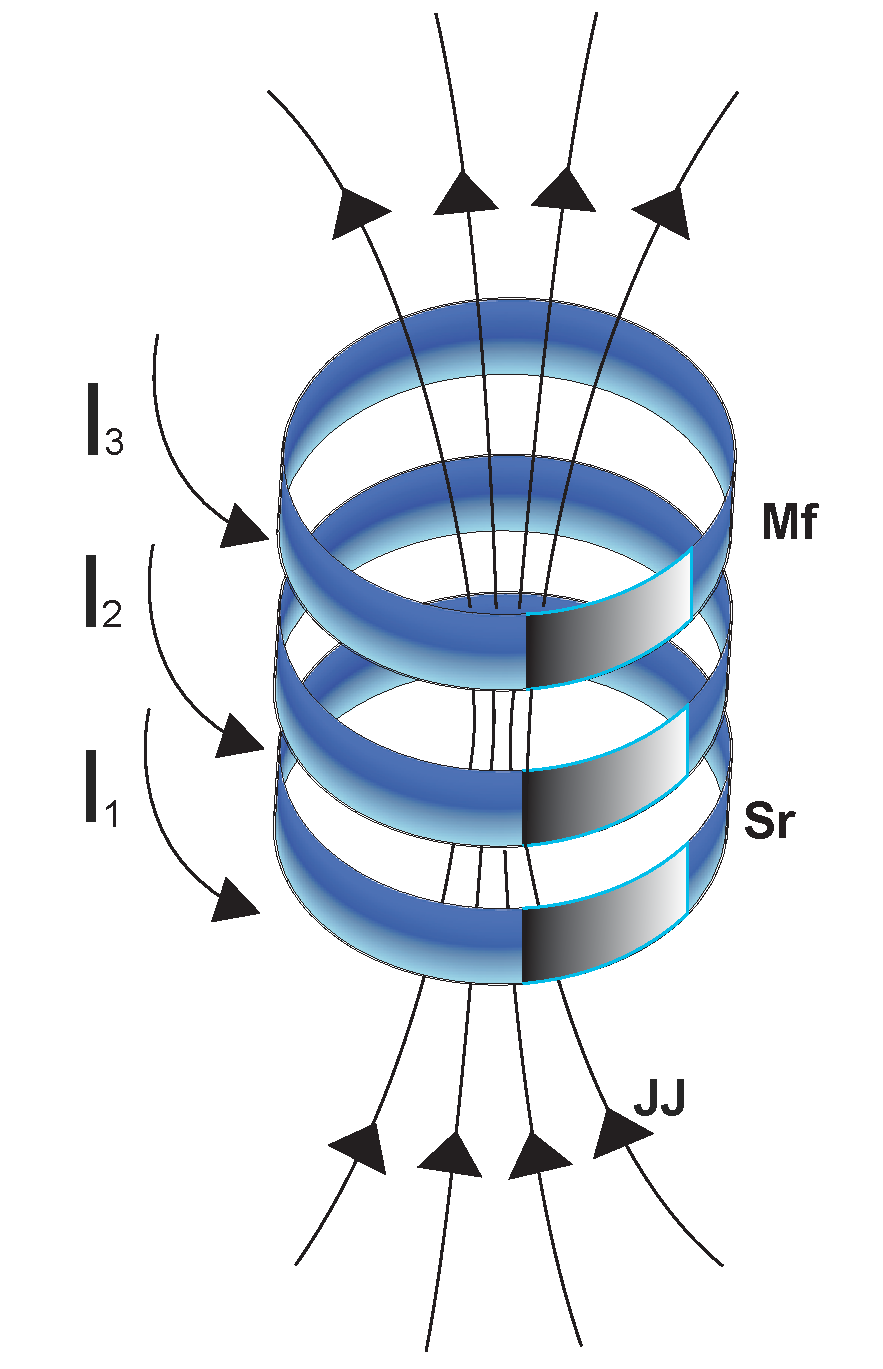
\includegraphics[scale=0.27]{Fig00}% Here is how to import EPS art
	\caption{ Schematic diagram of a SQUID trimer with  positive magnetic coupling strength,
		in a magnetic field where (Mf) is the Magnetic field, (Sr) is the Superconducting ring,
		(JJ) is the Josephson Junction, and ($I_{1}$), ($I_{2}$) and ($I_{3}$) are the induced currents.} \label{fig00}
\end{figure} 

\begin{figure*}
	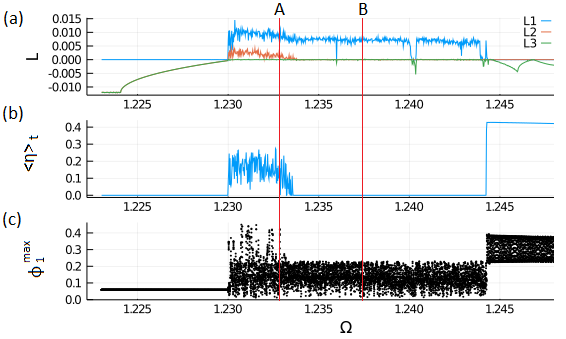
\includegraphics[scale=0.8]{Fig01}
	\caption{(a) The three maxima Lyapunov exponents (the rest are negative), (b) the mean value over time of $\eta$ and (c) maximum value of the magnetic flux $\phi_{1}$ as a function of the driving frequency. Red line A corresponds to $\Omega = 1.233$ and B to $\Omega = 1.2375$. We observe two main regions: The first one is between ($\Omega=1.23,\Omega=1.234$) corresponds to hyperchaos intermittent synchronization where ($\left\langle \eta\right\rangle _{t} < 0.3$, $L_{1} > 0$, $L_{2} > 0$, $L_{3} = 0$) and the second one lying between ($\Omega=1.234,\Omega=1.244$) corresponds to chaos synchronization where ($\left\langle \eta\right\rangle _{t} \simeq 0$, $L_{1} > 0$, $L_{2} =L_{3} = 0$). Parameters: $\lambda=0.1075$, $\phi_{ac}=0.02$, $\gamma=0.024$, $\phi_{dc}=0$ and $\beta=0.1369$.} \label{fig01}
\end{figure*} 

In order to quantify the synchronization between $\phi_{1}(t)$ and $\phi_{3}(t)$ we calculate the $\eta$ measurement \cite{Baker1998}:

\begin{equation} \label{}
\eta(t) =\sqrt{ (\phi_{1}(t)-\phi_{3}(t))^{2} + (\dot{\phi_{1}}(t)- \dot{\phi_{3}}(t))^{2} }, 
\end{equation}

where for $\eta$ in time close to zero we have almost perfect synchronization. Regarding the $\eta$ average over time, we have observed, after careful numerical calculations, that the dynamic relationship between $\phi_{1}(t)$ and $\phi_{3}(t)$ revels three main behaviors: Synchronization when $\left\langle \eta\right\rangle _{t} < 0.01$ in the interval between $\Omega=1.223$ and $\Omega=1.23$, intermittent synchronization when $0.01<\left\langle \eta\right\rangle _{t} < 0.3$ in the interval between $\Omega=1.23$ and $\Omega=1.234$ and no synchronized or unsynchronized solutions when $0.3 < \left\langle \eta\right\rangle _{t}$ in the interval between $\Omega=1.244$ and $\Omega=1.2475$ (Fig. \ref{fig01} (b)). It is remarkable, however, that synchronization can be achieved even in the chaotic regime between $\Omega=1.234$ and $\Omega=1.244$ where $L_{1}>0$ and $L_{2} = L_{3} \simeq 0$, as shown in Fig. \ref{fig01} (a) .
Finally, in Fig. \ref{fig01} (c) the maxima of the solution for $\phi_{1}(t)$ is plotted over $\Omega$. For this continuation only one set of different initial conditions were used, however the regions of periodic, hyperchaotic, chaotic and quasiperiodic solutions within the $\Omega$ interval are well observed.

We examine two main regions in our system by fixing the driving frequency $\Omega$
to a certain value. Hyperchaos and chaos have been marked by the red horizontal
line A and B (Fig. \ref{fig01}) and the temporal evolution in SQUID 1 and 3 have been plotted for the respective areas ($\Omega = 1.233$ and $\Omega = 1.2375$)  as shown in Fig. \ref{fig02} (a) and (b). Blue represents the first SQUID and red the third SQUID. For $\Omega = 1.233$, the time evolution of $\phi_{1}$ and $\phi_{3}$ are not synchronized (Fig. \ref{fig02} (a)) although, there are some windows in time where synchronization occurs. This is a hyperchaos intermittent synchronization and we will address this phenomena in more details in the next section. This unsynchronized behavior can be confirmed in both ($\phi_{1}$,$\phi_{2}$) and ($\phi_{1}$,$\phi_{3}$) plane projections (Fig. \ref{fig02} (c), (e)). Synchronized chaos can be seen in Fig. \ref{fig02} (b) as the time series of the trimer edges are identical. The projection of the flow onto the ($\phi_{1}$,$\phi_{3}$) plane confirm this behavior (Fig. \ref{fig02} (f)), in contrast with the ($\phi_{1}$,$\phi_{2}$) plane projection where no synchronization occurs (Fig. \ref{fig02} (d)).  







\begin{figure}
	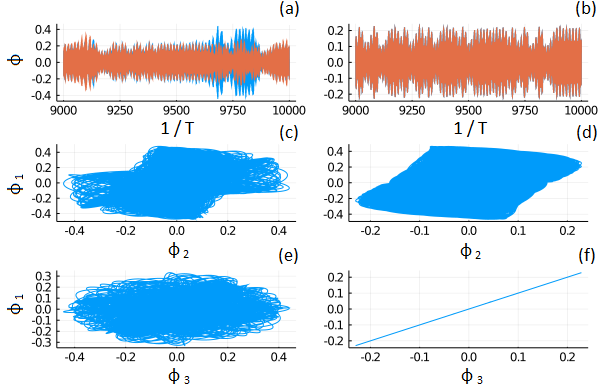
\includegraphics[scale=0.55]{Fig02}% Here is how to import EPS art
	\caption{Unsynchronized chaos for a set of parameters as in Fig. \ref{fig01} (A red line) where $ \Omega = 1.233$. (a) Time series for $\phi_{1}$ (blue color) and $\phi_{3}$ (red color). (c) Projection of the flow onto $\phi_{1}$ - $\phi_{2}$ plane. (e) Projection into the $\phi_{1}$ - $\phi_{3}$ plane. (b), (d) and (f) the same for synchronized chaos where the set of parameters as in Fig. \ref{fig01} (B red line) where $\Omega = 1.2375$.} \label{fig02}
\end{figure}


\section{The parameter space}

\begin{figure*}
	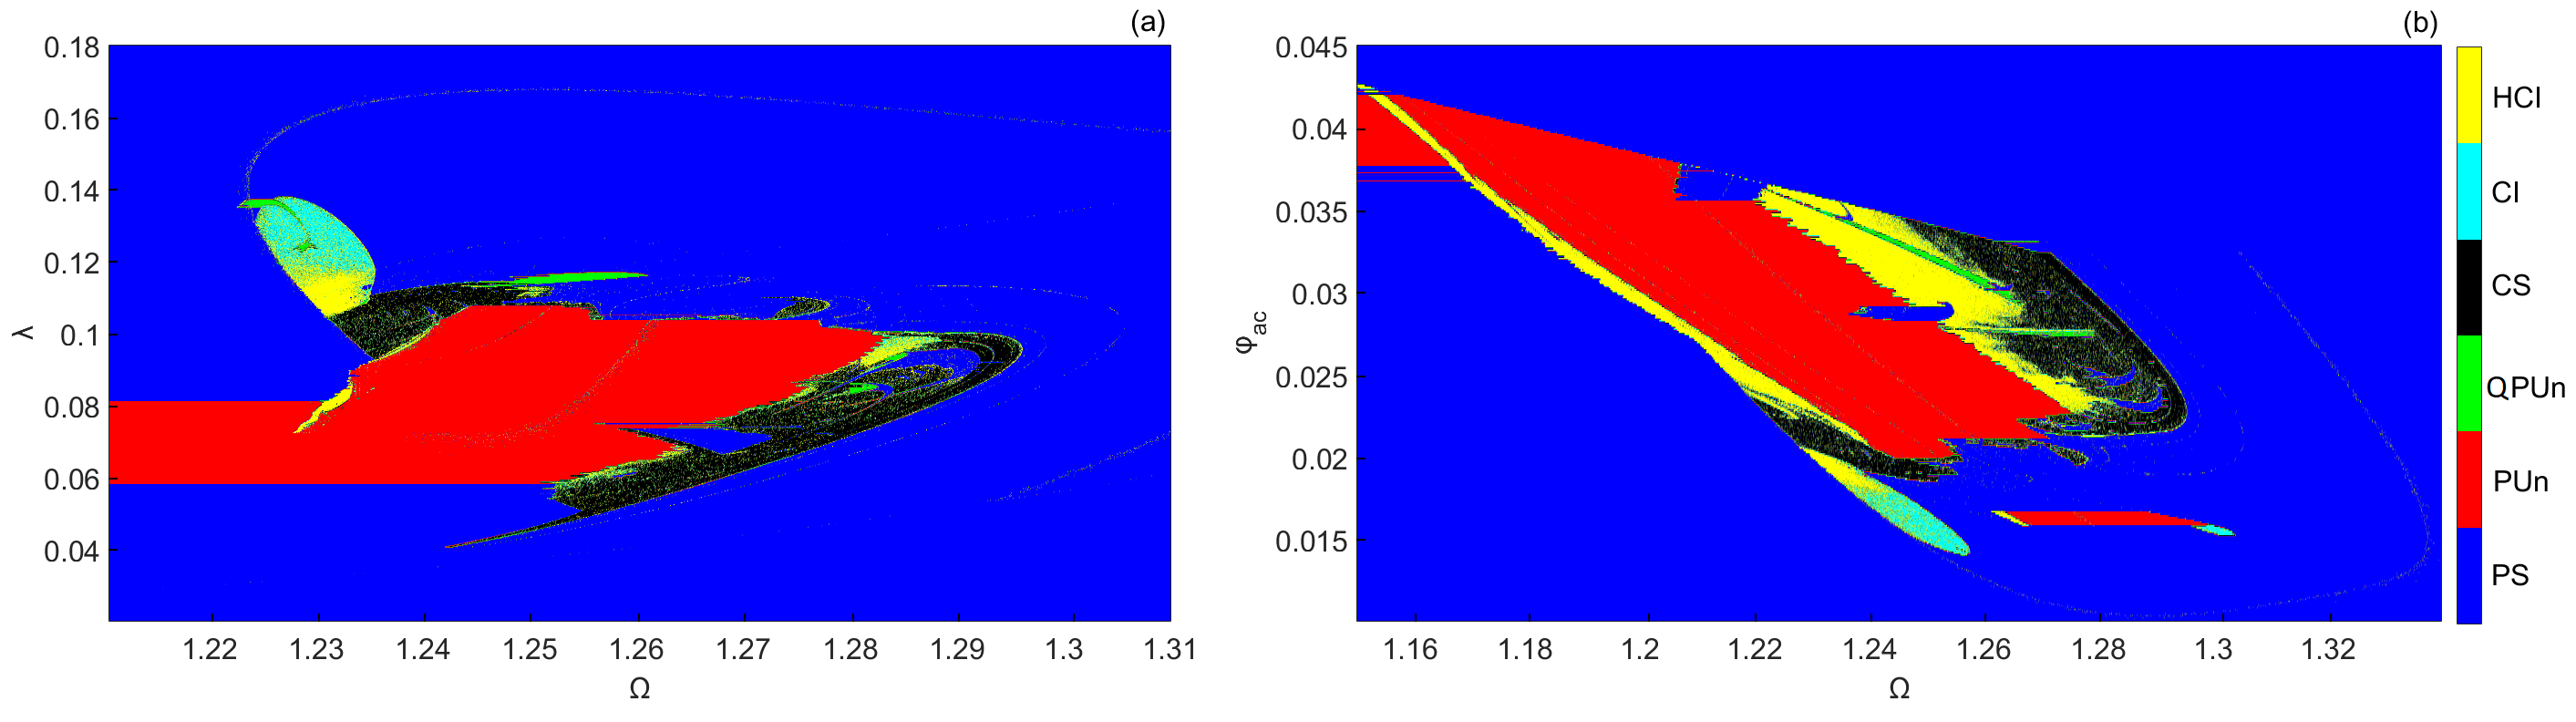
\includegraphics[scale=0.25]{Fig03}
	\caption{Map of different dynamical regions in the (a) ($\lambda$,$\Omega$) parameter space where $\phi_{ac} = 0.02$ and (b) in the ($\phi_{ac}$,$\Omega$) parameter space where $\lambda = 0.02$. Depending on three maxima Lyapunov exponents ($L_{1}>L_{2}>L_{3}$) and $\left\langle \eta\right\rangle _{t}$ quantifier, we observe six different areas. 
	Periodic synchronization (PS), Periodic Unsynchronized solutions (PUn), 
	Quasiperiodic unsynchronized solution (QPUn), 
	Chaos synchronization (CS), 
	Chaos intermittent synchronization (CI) and finally 
	Hyperchaos intermittent synchronization (HCI). Other parameters: $\gamma=0.024$, $\phi_{dc}=0$ and $\beta=0.1369$.} \label{fig03}
\end{figure*}

As we mentioned early, for the $\eta$ average over time, we observe three main behaviors: Synchronization, intermittent synchronization and no synchronized or unsynchronized solutions. Moreover, by calculating the Lyapunov exponents we have periodic solutions, quasiperiodicity, chaos and hyperchaos. In Fig.\ref{fig03}, a map of different dynamic regions in combination with $\left\langle \eta\right\rangle_{t}$ and maxima Lyapunov exponents are shown in ($\Omega$,$\lambda$) (Fig.\ref{fig03} (a)) and ($\Omega$,$\phi_{ac}$) (Fig.\ref{fig03} (b)) parameter space. We observe six different areas. Periodic synchronization (PS) where $L_{1}=0, L_{2}, L_{3} <0$ and $\left\langle \eta\right\rangle _{t} < 0.01$, periodic unsynchronized solution (PUn)  where $L_{1}=0, L_{2}, L_{3} <0$ and $0.3<\left\langle \eta\right\rangle _{t}$, quasiperiodic unsynchronized solution (QPUn) where $L_{1}=L_{2}=0, L_{3}<0$ and $\left\langle \eta\right\rangle _{t} > 0.3$, chaos synchronization (CS) where $L_{1}>0,L_{2}=L_{3}=0$ and $\left\langle \eta\right\rangle _{t} < 0.01$, chaos intermittent synchronization (CI)  where $L_{1}>0,L_{2}=L_{3}=0$ and $0.01<\left\langle \eta\right\rangle _{t} < 0.3$ and finally hyperchaos intermittent synchronization (HCI) where $L_{1}>0,L_{2}>0,L_{3}=0$ and $0.01<\left\langle \eta\right\rangle _{t} < 0.3$.

Both in the parameter interval ($\Omega$,$\lambda$) and ($\Omega$,$\phi_{ac}$), periodic synchronization (PS) occupies most of the surface. Next, the main dynamic behavior is concentrated in a periodic unsynchronized solution (PUn). At the boundaries of this region, we observe chaos synchronization (CS) and hyperchaos intermittent synchronization (HCI). It is remarkable that hyperchaos always appears with intermittent synchronization of $\phi_{1}(t)$ and $\phi_{3}(t)$. We have never observed synchronization or unsynchronized solutions between the trimer edges, in the presence of hyperchaos. The opposite is not true. Indeed, intermittent synchronization can also be observed in the chaotic regime (Fig.\ref{fig03}, Maya blue color (CI)). Finally, very small areas of quasiperiodic unsynchronized solutions (QPUn) fill the parameter space.

Three specific dynamic regions of non chaotic behavior are shown in Fig. \ref{fig04} with constant $\phi_{ac} = 0.02$. The time series of the magnetic flux (Fig. \ref{fig04} (a) first column), for $\Omega = 1.21$ and $\lambda=0.16$, show a periodic synchronization between the first (red color) and third (blue color) SQUID. The time series of $\eta$ close to zero also indicate a synchronization behavior (Fig. \ref{fig04} (a) second column). When $\Omega = 1.24$ and $\lambda=0.07$, $\phi_{1}(t)$ and $\phi_{3}(t)$ oscillate out of phase, with different amplitudes, where $\eta$ also oscillate over time with an average time value greater than $0.3$, an indication for a periodic unsynchronous solution (Fig. \ref{fig04} (b) first and second column). For $\Omega = 1.255$ and $\lambda=0.118$, the temporal evolution of the system is quasiperiodic and the magnetic flux of the first and third SQUIDs oscillates in time with different frequencies and amplitudes (Fig. \ref{fig04} (c) first column). The $\eta$ quantifier also has a period evolution with multiple frequencies due to the quasiperiodic behavior, where $ 0.3 < \left\langle \eta\right\rangle _{t}$ as an evident of non-synchronization between the trimer edges.

Figure. \ref{fig05} illustrates three other dynamic examples, this time in the chaotic regime. For $\Omega = 1.235$ and $\lambda=0.1$ the temporal evolution of the system is chaotic and the output magnetic fluxes in SQUID 1 and 3 are identical, as shown in Fig. \ref{fig05} (a), first column. This chaotic synchronization is confirmed by the evolution of $\eta$ close to zero in the second column. When  $\Omega = 1.23$ and $\lambda=0.125$ the time series of the trimer edges are chaotic but not identical. The three maxima Lyapunov exponents associated with this evolution are ($+0.007, -3.3e-5, +1.7e-5$). Nevertheless, there are some windows in time where synchronization occurs (Fig. \ref{fig05} (b), first column). This is a chaos intermittent synchronization where $\eta$ evolves, at some temporal intervals close to zero (synchronous behavior) and at others with large fluctuations between zero and one (Fig. \ref{fig05} (b), second column). The same dynamic behavior as the previous is demonstrated in Fig. \ref{fig05} (c) for both $\phi_{1}(t)$ and $\phi_{3}(t)$ (first column) and $\eta$ quantifier (second column) where $\Omega = 1.23$ and $\lambda=0.11$. However, in this case, the associated three maxima Lyapunov exponents are ($+0.015, +0.002, -6.7e-6$). The system is now hyperchaotic, with more than one positive Lyapunov exponent and so the behavior of the system is characterized as hyperchaotic intermittent synchronization.       







 


\begin{figure}
	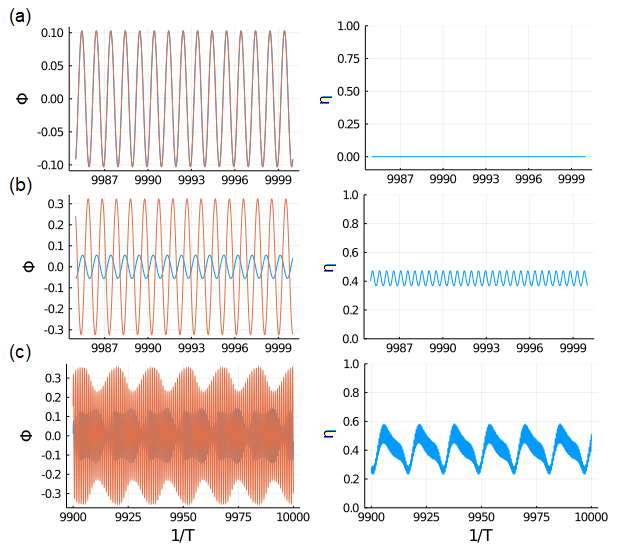
\includegraphics[scale=0.55]{Fig04_A}% Here is how to import EPS art
	\caption{(a) Periodic synchronization (PS) where $\Omega = 1.21$ and $\lambda=0.16$. (b) Periodic unsynchronized (PUn) solution where $\Omega = 1.24$ and $\lambda=0.07$ (c) Quasiperiodic unsynchronized (QPUn) solution where $\Omega = 1.255$ and $\lambda=0.118$. In first column the time series of the magnetic flux for the first SQUID, (red line), and the third SQUID, (blue line). In second column $\eta$ over time. Other parameters: $\phi_{ac}=0.02$, $\gamma=0.024$, $\phi_{dc}=0$ and $\beta=0.1369$.} \label{fig04}
\end{figure}

\begin{figure}
	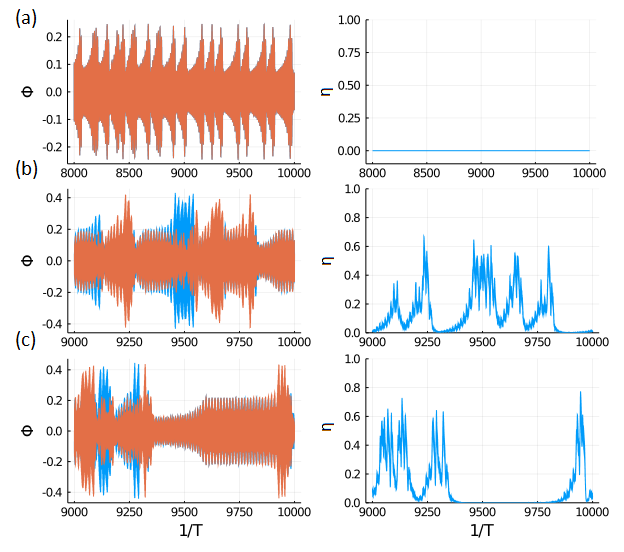
\includegraphics[scale=0.55]{Fig04_B}% Here is how to import EPS art
	\caption{(a) Chaos synchronization (CS) where $\Omega = 1.235$ and $\lambda=0.1$. (b) Chaos intermittent synchronization (CI) where $\Omega = 1.23$ and $\lambda=0.125$. (c) Hyperchaos intermittent synchronization (HCI) where $\Omega = 1.23$ and $\lambda=0.11$. First and second column as in Fig.\ref{fig04}. Other parameters: $\phi_{ac}=0.02$, $\gamma=0.024$, $\phi_{dc}=0$ and $\beta=0.1369$.} \label{fig05}
\end{figure}




%%%%%%%%%%%%%%%%%%%%%%%%%%%%%%%%%%%%%%%%%%%%%%%%%%%%%%%%%%%%%%

\section{CONCLUSIONS}\label{real}


\section{ACKNOWLEDGEMENTS}
This work was supported by the Ministry of Education and Science of the Russian Federation in the framework of the Increase Competitiveness Program of NUST ``MISiS'' (Grant number K4-2018-049).

\bibliography{bibliography}

\end{document}